%!TEX root = ../main.tex
%%%%%%%%%%%%%%%%%%%%%%%%%%%%%%%%%%
% Links:
%
% Difficulty:
% Companies: 
%%%%%%%%%%%%%%%%%%%%%%%%%%%%%%%%%%

\chapter{Median of two sorted arrays}
\label{ch:median_sorted_arrays}
\section*{Introduction}

The problem presented in this chapter is considered a hard one to solve optimally. Nevertheless is has been asked countless times in coding interviews, and for this reason we should be able to solve it in a reasonable amount of time. Despite the optimal solution (logarithmic time and constant space) can be difficult to achieve, this problem can be solved fairly easily and quickly in suboptimal ways. We suggest not to dive into those suboptimal approaches because the interviewer is expecting the optimal solution for this problem, but to just mention quickly one of them at the beginning.


\section{Problem statement}
\begin{exercise}
There are two sorted arrays $A$ and $B$ of size $m$ and $n$ respectively.

Find the median of the two sorted arrays. The overall run time complexity should be O(log (m+n)).

You might assume that $n+m > 0$

	\begin{example}
		\hfill \\
		Given two sorted arrays:
		\begin{itemize}
			\item $A=[1,4,6,10]$
			\item $B=[2,3,5,6]$
		\end{itemize}
		The median is $\frac{5+4}{2} = 4.5$ (see Figure \ref{fig:median_sorted_arrays:example1}).

		See Figure \ref{fig:median_sorted_arrays:example2} for an example where the total number of elements in the two arrays is odd.
	\end{example}

\end{exercise}

\begin{figure}
	\label{fig:median_sorted_arrays:example1}
	\centering
	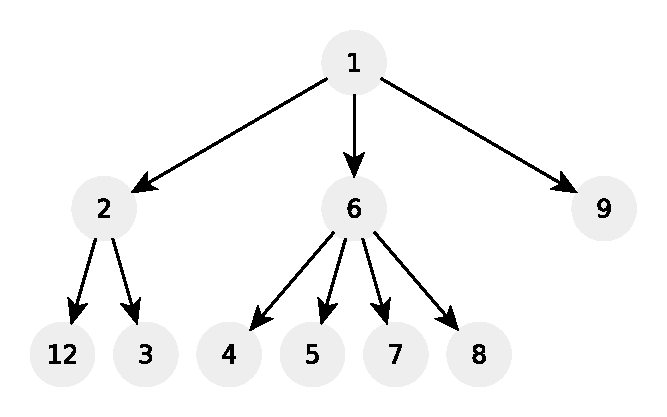
\includegraphics[scale=1.0]{sources/median_sorted_arrays/images/example1}
	\caption{Example of median of two sorted array.}
\end{figure}

\begin{figure}
	\label{fig:median_sorted_arrays:example2}
	\centering
	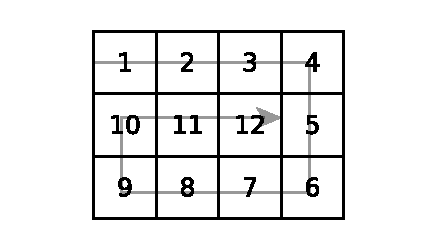
\includegraphics[scale=1.0]{sources/median_sorted_arrays/images/example2}
	\caption{Example of median of two sorted array.}
\end{figure}

%\section{Clarification Questions}
%
%\begin{QandA}
%	\item 
%	\begin{answered}
%		\textit{}
%	\end{answered}
%	
%\end{QandA}

\section{Discussion}
\label{median_sorted_arrays:sec:discussion}
Let's start our discussion by reviewing the concept of median.
The median of a collection $C$ of $n$ elements is:
\begin{itemize}
	\item $C_{\frac{n}{2}}$ if $n$ is odd (see Figure \ref{fig:median_sorted_arrays:example1})
	\item $\frac{C_{\floor{\frac{n}{2}}}+C_{\ceil{\frac{n}{2}}}}{2}$ if $n$ is even (see Figure \ref{fig:median_sorted_arrays:example2})
\end{itemize}
In simpler terms the median of a sorted collection is the element which  divides the collections into two equal parts, left and right, each with the same number of elements. If $n$ is even clearly this element does not exists and thus the median is the calculated using the two middle elements as in Figure \ref{fig:median_sorted_arrays:example1}. Additionally, for this problem we are looking for the median of a sorted data, hence, it also has a nice property that all the elements on its left side are smaller and on the right side greater. 

\subsection{Brute-force}
\label{median_sorted_arrays:sec:bruteforce}
Armed with the definition of median, we can immediately devise a simple and effective approach to calculate it given two sorted array. The very first thing that should come to mind is to 
\begin{enumerate}
	\item  create an array $C = A+B$, which is the concatenation of the two input arrays
	\item sort $C$
	\item calculate the median depending on the parity of $C$
\end{enumerate}

This approach is correct (see its implementation in Listing \ref{list:median_sorted_naive}), but it is far from being optimal. Given $s$ is the size of $C$ i.e. $s=n+m$, the time and space complexities of this approach are $O(nlog(n))$ and $O(n)$, respectively.

\lstinputlisting[language=c++, caption={Naive implementation of solution to the problem of finding the median of two sorted arrays.},label=list:median_sorted_naive]{sources/median_sorted_arrays/median_sorted_arrays_solution1.cpp}


\subsection{Brute-force improved}
\label{median_sorted_arrays:sec:bruteforce_improved}
The brute-force approach can be improved a bit if we use the fact that the arrays are already sorted. In the approach described in Section \ref{median_sorted_arrays:sec:bruteforce} we do not use this fact and therefore we are forced to sort the array $C$. This is not necessary if the input arrays are sorted already because we can merge the two inputs in linear time. This is basically the same operation that is one of the basic building block of the merge-sort algorithm\cite{wiki:mergesort}. Listing \ref{list:median_sorted_naive_2} shows a possible implementation of this idea together with an implementation of the sorted array merge function. 

\lstinputlisting[language=c++, caption={Naive implementation of solution to the problem of finding the median of two sorted arrays using the merge part of merge-sort algorithm.},label=list:median_sorted_naive_2]{sources/median_sorted_arrays/median_sorted_arrays_solution2.cpp}

The time complexity of this version, $O(n+m)$ is better than the one from the solution presented in Section \ref{median_sorted_arrays:sec:bruteforce} but it is still suboptimal. This problem can be solved in logarithmic time. We are going to see how in Section \ref{median_sorted_arrays:sec:log}.

\subsection{Logarithmic solution}
\label{median_sorted_arrays:sec:log}
Let's start by pointing out that the very essence of this problem is to try to figure out how the merging the two arrays together into one would look like (like in the previous sections) but without actually performing the merging itself.

The key ideas are:
\begin{itemize}
	\item we know exactly how big is the merged array ($C$)
	\item the left part of $C$, $C_l$ would be made up from portions of the smallest values of $A$ and $B$. For instance, w.r.t. the example in Figure \ref{fig:median_sorted_arrays:example2} we can see that the left half (the first $5$ elements) of $A+B$ is made from the first two elements of $A$ and the smallest $3$ elements of $B$. Because $C$ will be sorted, only the smallest elements of $A$ and $B$ will contribute to its left half.
\end{itemize}

At the beginning we do not know exactly how many elements from $A$ will be part of the first half of $C$, $C_l$. But we can try to search for this number. 
Let's suppose we try to construct $C_l$ by using $i$ elements from $A$. Because we know the size of $C$ i.e. $s=n+m$ (the sum of the sizes of $A$ and $B$), we also know the size of $C_l$, $s_2 = \frac{s}{2}$. Thus, we also know how many elements we need to take from the left part of $B$ ($B_l$), i.e. $s_2 - i$.
